\documentclass{article}
\usepackage[utf8]{inputenc}
\usepackage{pgfplots}

\title{Kvadratické funkcie}
\author{Michal Špano}
\date{October 2021}

\begin{document}
\maketitle
\section{Príklad 1}

% Define exercise
Majme funkciu $f(x): y = 2x^2+8x+4$, nájdime $g(x)$, ktorej graf je osovo súmerný s grafom $f(x)$ podľa $y=-1$.\-

% Solution
Úlohou je dostať funkciu do tvaru: $f(x): y = (x-V_x)^2 + V_y$,\\kde $V[V_x, V_y]$ predstavuje vrchol paraboly.
\[ f(x): y = 2x^2+8x+4 \] 
\begin{center}\textbf{…}\end{center} 
\[ f(x): y = 2(x+2)^2-4 \Rightarrow V[-2;-4] \]
Vzdialenosť $V_y=-4$ od $y=-1$, t.j. $|-1-4|=3$ nám určí, že $V'$, teda vrchol paraboly $g(x)$ leží v bode $V'_y=2$. \\

% Graphical depiction
\textbf{Graficky:}

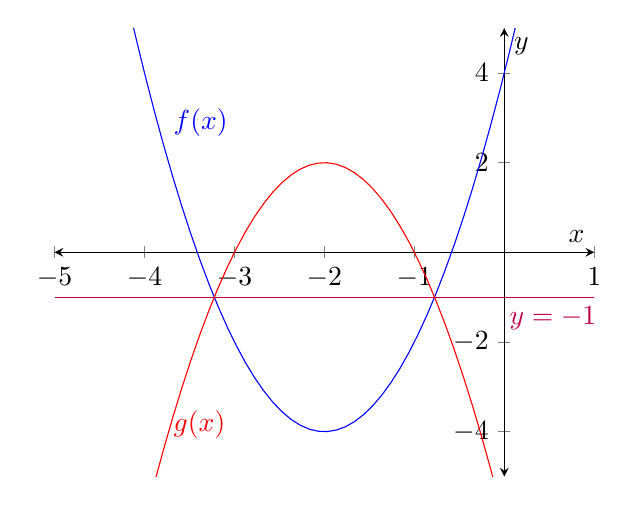
\begin{tikzpicture}[>=stealth]
    \begin{axis}[
        xmin=-5,xmax=1,
        ymin=-5,ymax=5,
        axis x line=middle,
        axis y line=middle,
        axis line style=<->,
        xlabel={$x$},
        ylabel={$y$},
        ]
        \addplot[no marks,blue,<->] expression[domain=-5:5,samples=100]{2*(x+2)^2-4} 
                    node[pos=0.1, anchor=south west]{$f(x)$};
        \addplot[no marks,red,<->] expression[domain=-5:5,samples=100]{-2*(x+2)^2+2} 
                    node[pos=0.1, anchor=south west]{$g(x)$};
        \addplot[purple] expression[domain=-5:5, samples=100]{-1}
                    node[pos=0.495, anchor=north west]{$y=-1$};
    \end{axis}
\end{tikzpicture}
\end{document}

